\section{Lecture 18 -- 15th November 2023}
Today, we consider yet another example of infinity categories that arises in the study of cobordisms of manifolds. 
\begin{definition}[Cobordism]\label{def: cobordism}
    Let $M,N$ be $n$-manifolds. A cobordism between $M$ and $N$ is an $(n+1)$-manifold $W$ such that $\partial W=M\sqcup N$. 
\end{definition}
\begin{figure}[h]
    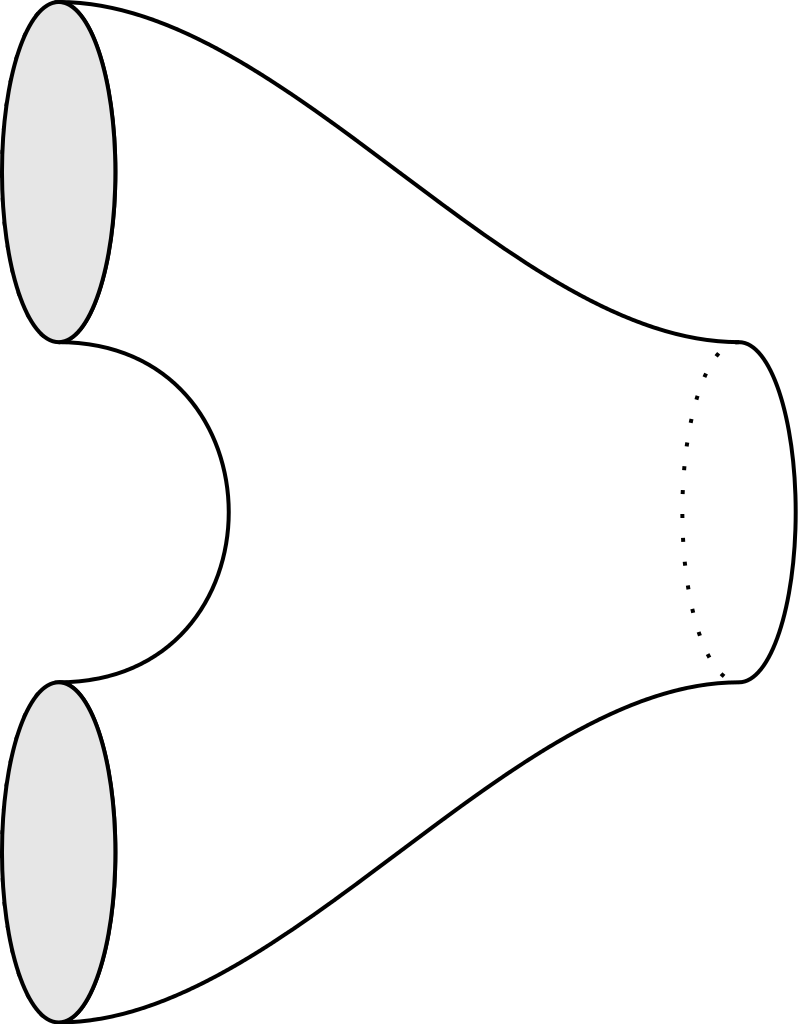
\includegraphics[width=3cm]{Pants.png}
    \label{fig: pair of pants}
    \caption{The pair of pants is a cobordism between $S^{1}$ and $S^{1}\sqcup S^{1}$.}
\end{figure}
This first arose in Pontryagin's study of manifolds and remains an active area of research to this day. Let $\Omega^{n}$ be the cobordism classes of $n$ manifolds. This naturally forms a monoid under the operation of disjoint union with identity element $\emptyset$. $\Omega^{n}$ can naturally be endowed with the structure of a group by noticing that $M\sqcup M$ is cobordant to $\emptyset$ by identifying the boundary of $M\times[0,1]$ yielding an $(n+1)$-manifold without boundary. \\\\
In the late 1980s, physicists were concerned about string theory, which encouraged the study of cobordisms that were treated as non-invertible transformations. This led to the definition of a cobordism category and topological quantum field theory. In particular, we define the bordism category as follows. 
\begin{definition}[$\Bord_{(n-1,n)}$]
    The category $\Bord_{(n-1,n)}$ has objects $(n-1)$-manifolds with morphisms cobordism and a composition law given by concatenation. 
\end{definition}
This definition leads to a problem. In concatenation, one must choose an appropriate open neighborhood of the boundaries of the $n$-manifolds. Different choices of open neighborhoods yield to different concatenated manifolds. In particular, the composition is not associative, but is associative up to diffeomorphism in a non-cannonical way. This leads us to believe that there is higher structure, in particular the structure of a symmetric monoidal category. 
\begin{definition}[Symmetric Monoidal Category]\label{def: symmetric monoidal category}
    A symmetric monoidal category $\Csf$ is a category $\Csf$ with a functor $\otimes:\Csf\times\Csf\to\Csf$ and an object $1_{\Csf}\in\Obj(\Csf)$ such that the following conditions are fulfiled: 
    \begin{enumerate}[label=(\alph*)]
        \item A natural isomorphism $1_{\Csf}\otimes 1_{\Csf}\to 1_{\Csf}$. 
        \item For all $A\in\Obj(\Csf)$, a natural isomorphisms $1_{\Csf}\otimes A\to A$ and $A\otimes 1_{\Csf}\to A$.
        \item For all $A,B\in\Obj(\Csf)$, a natural isomorphism $A\otimes B\to B\otimes A$. 
        \item For all $A,B,C\in\Obj(\Csf)$, a natural isomorphism $(A\otimes B)\otimes C\to A\otimes(B\otimes C)$. 
    \end{enumerate}
\end{definition}
One can check that $\sqcup$ defines an operation that satisfies the symmetric monoidal structure on $\Bord_{(n-1,n)}$ with $1_{\Bord_{(n-1,n)}}=\emptyset$. This leads to the definition of a topological quantum field theory. 
\begin{definition}[Topological Quantum Field Theory]
    A topological quantum field theory is a symmetric monoidal functor $\Bord_{(n-1,n)}\to\Csf$ for $\Csf$ a symmetric monoidal category. 
\end{definition}
For our discussion today, we consider $\Csf=\Vect_{\CC}$ yielding a functor $Z:\Bord_{(n-1,n)}\to\Vect_{\CC}$ taking an $(n-1)$-manifold $M$ to a $\CC$-vector space $Z(M)$ such that $Z(M_{1}\sqcup M_{2})\mapsto Z(M_{1})\otimes Z(M_{2})$ with unit $\emptyset$ in $\Bord_{(n-1,n)}$ to $Z(\emptyset)=\CC$. Suppose $N$ is an $n$-manifold defining a cobordism between $(n-1)$-manifolds $M_{1}$ and $M_{2}$. This yields a linear map of $\CC$-vector spaces $Z(M_{1})\to Z(M_{2})$. For $N$ a boundaryless $n$-manifold, $N$ is a cobordism between $\emptyset$ and $\emptyset$, hence $Z(N)$ is a map $\CC\to \CC$ by $1\mapsto\lambda$ for $\lambda\in\CC$. In such a case, it suffices to study this value $\lambda$. 
\\\\
Further restricting our case to oriented 1-manifolds up to cobordism by 2-manifolds, we consider the category $\Bord_{(1,2)}^{\mathrm{so}}$. Recall from a course in topology that a closed 1-manifold is the disjoint union of $S^{1}$s, and thus $Z(S^{1})$ is some $\CC$-vector space $V$. The upper half sphere gives a cobordism between $S^{1}$ and $\emptyset$, yielding a trace $V\to\CC$. In the case of cobordisms of 1-manifolds, there is a clear interpretation of the relavent topological quantum field theory. 
\begin{theorem}
    Symmetric monoidal functors $Z:\Bord_{(2,1)}^{\mathrm{so}}\to\Vect_{\CC}$ correspond to Frobenius algebras. 
\end{theorem}
Symmetric monoidal categories therefore define another model for $\infty$-categories that are used in the study of topological quantum field theories. These may seem idiosyncratic, but really are the most morally correct way to study these mathematical structures. Work in this area continues to this day, with a recent landmark result by Lurie in his solution of the Baez-Dolan Cobordism hypothesis, characterizing these cobordism categories by universal higher categorical structures. See the survey article by Freed \cite{Freed} for a brief overview and the papers by Ayala-Francis \cite{AyalaFrancis} and Grady-Pavlov \cite{GradyPavlov} for more information. 
\\\\
Let us now consider yet another approach to higher category theory. Let $\Csf$ be a category. Let's think about this category via the moduli space of functors to it. 
\begin{definition}[Maximal Groupoid]
    Let $\Csf$ be a category. The maximal groupoid in $\Csf$, denoted $\Csf^{\sim}$, is the maximal subcateory of $\Csf$ in which every morphism is an isomorphism. 
\end{definition}
Evidently $N\Csf^{\sim}$ is a Kan complex by Joyal's horn filling condition \Cref{thm: Joyal extension theorem}. This is the moduli space of objects of $\Csf$ in the sense that when we treat $N\Csf^{\sim}$ as a topological space, the connected components are isomorphism classes of objects. Similarly for $I$ an indexing category, $N(\Csf^{I})^{\sim}$ is the moduli space of $I$-diagrams in $\Csf$. We can probe this object by taking $I=[n]$ defining a functor $\DDelta\to N(\Csf^{\DDelta})^{\sim}$ by $[n]\mapsto N(\Csf^{[n]})^{\sim}$ valued in simplicial (topological) spaces. This led to the introduction of complete Segal spaces by Rezk. 
\begin{definition}[Segal Space; Rezk]\label{def: segal space}
    Let $X$ be a simplicial set. $X$ is a Segal space if for all $n$ if the Segal map $X^{\Delta_{n}}\to X^{I_{n}}$ induced by the spine inclusion $I_{n}\to\Delta^{n}$ given by 
    $$X_{n}\to\underbrace{X_{1}\times_{X_{0}}X_{1}\times_{X_{0}}\dots\times_{X_{0}}X_{1}}_{n\text{ times}}$$
    is an acyclic Kan fibration. 
\end{definition}
We can think of Segal spaces as a type of category whose objects are $X_{0}$ any two objects $A,B\in X_{0}$ we can define the space of maps between them as a pullback in the following diagram where $X\to X_{0}\times X_{0}$ is fibration 
$$% https://q.uiver.app/#q=WzAsNSxbMCwwLCJYXnsoQSxCKX0iXSxbMCwxLCIqIl0sWzIsMSwiWF97MH1cXHRpbWVzIFhfezB9Il0sWzIsMCwiWCJdLFswLDNdLFsxLDIsIihBLEIpIiwyXSxbMywyLCIoXFxsYW5nbGUwXFxyYW5nbGUsXFxsYW5nbGUxXFxyYW5nbGUpIl0sWzAsM10sWzAsMV1d
\begin{tikzcd}
	{X^{(A,B)}} && X \\
	{*} && {X_{0}\times X_{0}}
	\arrow["{(A,B)}"', from=2-1, to=2-3]
	\arrow["{(\langle0\rangle,\langle1\rangle)}", from=1-3, to=2-3]
	\arrow[from=1-1, to=1-3]
	\arrow[from=1-1, to=2-1]
\end{tikzcd}$$
and the space of map is denoted $X^{(A,B)}$. 
\begin{definition}[Complete Segal Space; Rezk]
    A segal space is complete if $X_{0}\to X_{1}^{\sim}$ is a homotopy equivalence of topological spaces where $X_{1}^{\sim}$ is the subset of isomorphisms in $X$. 
\end{definition}
Further work by Rezk and Joyal and Tierney relate complete Segal spaces to $\infty$-categories and quasicategories, respectively. 
\\\\
Returning to cobordism, we can let $X$ be a Segal space such that the $X_{0}$ correspond to closed $(n-1)$-manifolds. One can then show that 
$$X_{0}=\left\{S\subseteq\RR^{\infty}:S \text{ is a closed }(n-1)\text{-manifold}\right\}$$
and more generally
$$X_{n}=\left\{S\subseteq\RR^{\infty}\times\RR: S\text{ an }n\text{-manifold such that }\pi_{2}\text{ is proper and regular at }0,1,\dots,n\right\}.$$
Those more interested in this particular topic can refer to \cite{CalaqueScheimbauer}.